\chapter{Unit of Work}

\section{Caller Registration}

\begin{center}
    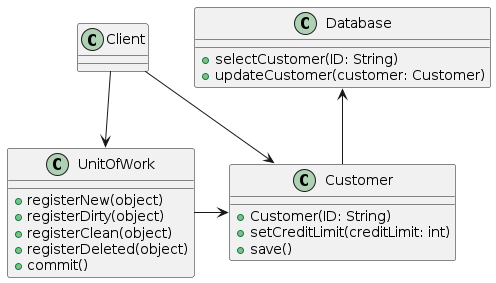
\includegraphics[width=12cm]{images/unit-of-work/CallerRegistrationClass.png}
\end{center}

\begin{center}
    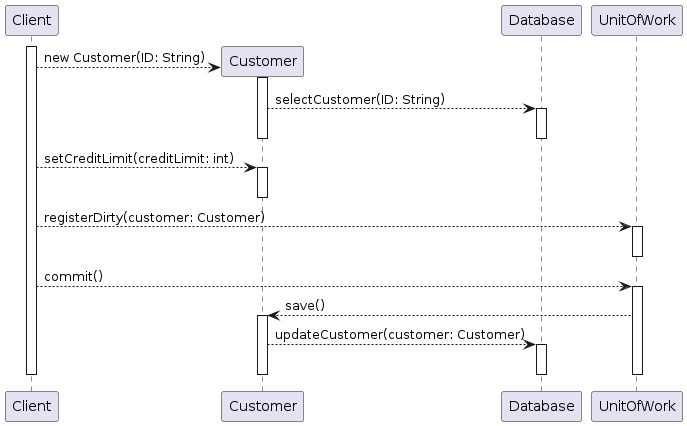
\includegraphics[width=12cm]{images/unit-of-work/CallerRegistrationSD.png}
\end{center}

Qui il Client ha il compito di informare UnitOfWork che l'oggetto Customer ha subito un cambiamento.
Il Client effettua il commit quando lo ritiene oppurtuno.

\section{Object Registration}

\begin{center}
    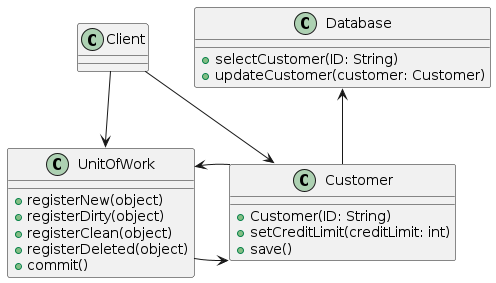
\includegraphics[width=12cm]{images/unit-of-work/ObjectRegistrationClass.png}
\end{center}

\begin{center}
    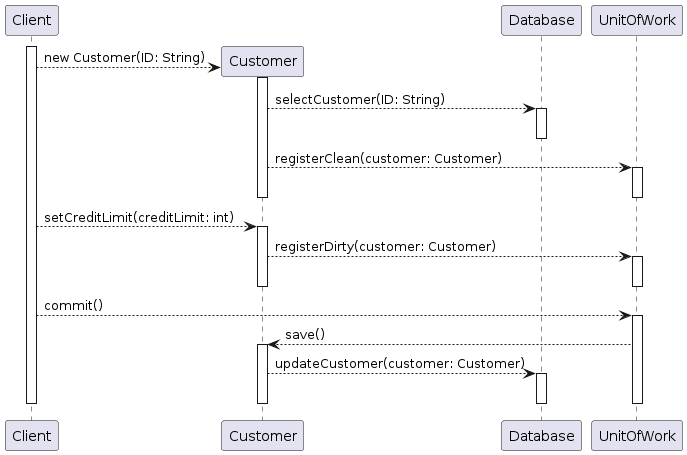
\includegraphics[width=12cm]{images/unit-of-work/ObjectRegistrationSD.png}
\end{center}

Qui invece e' l'oggetto Customer a registrare i propri cambiamenti al
Il Client effettua il commit quando lo ritiene oppurtuno.

\section{Controller}

\begin{center}
    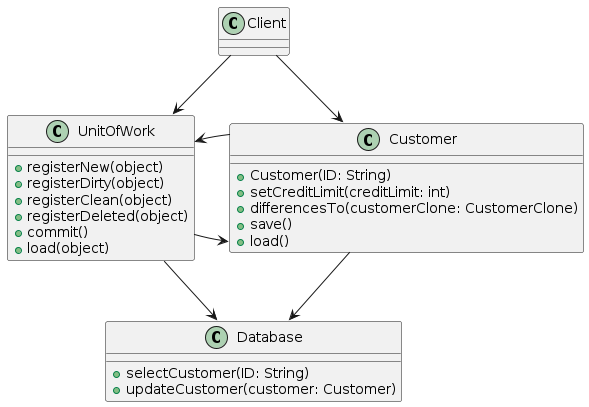
\includegraphics[width=12cm]{images/unit-of-work/ControllerClass.png}
\end{center}

\begin{center}
    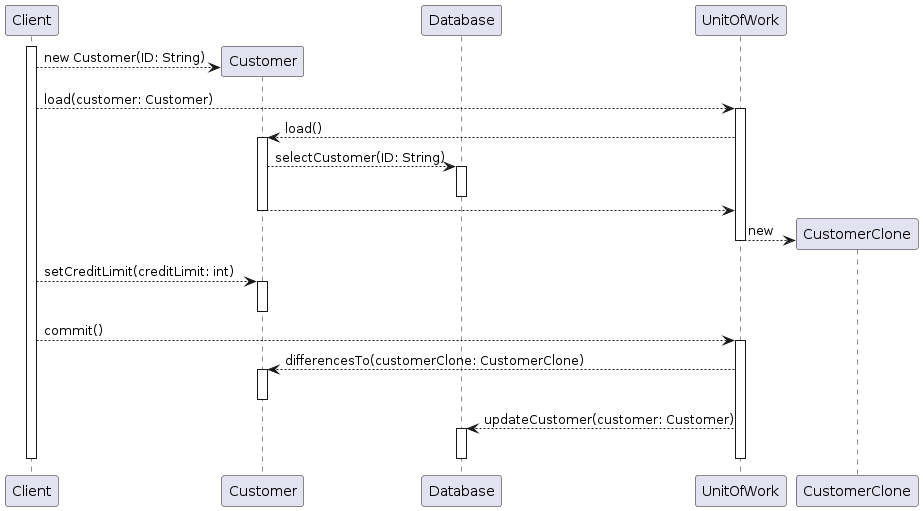
\includegraphics[width=16cm]{images/unit-of-work/ControllerSD.png}
\end{center}

Qui UnitOfWork e' notificata solo al momento della creazione dell'oggetto e si occupera' successivamente di controllare se un oggetto presenta cambiamenti che necessitano di essere salvati.
Si noti che qui UnitOfWork interagisce attivamente con il Database per aggiornare i dati. E' qui che essa ha l'opportunita' di gestire in modo ottimizzato le operazioni di scrittura.
Il Client effettua il commit quando lo ritiene oppurtuno.
